\documentclass{article}
% main document, called main.tex
\usepackage{tikz}
\usetikzlibrary{external}

\usetikzlibrary{positioning}
\usetikzlibrary{calc}
\usetikzlibrary{shapes.geometric, arrows, arrows.meta}
\usepackage{varwidth}% http://ctan.org/pkg/varwidth
\usetikzlibrary{shadows,trees, mindmap}
\usetikzlibrary{matrix}
\usetikzlibrary{fit}

\tikzexternalize % activate!

\begin{document}

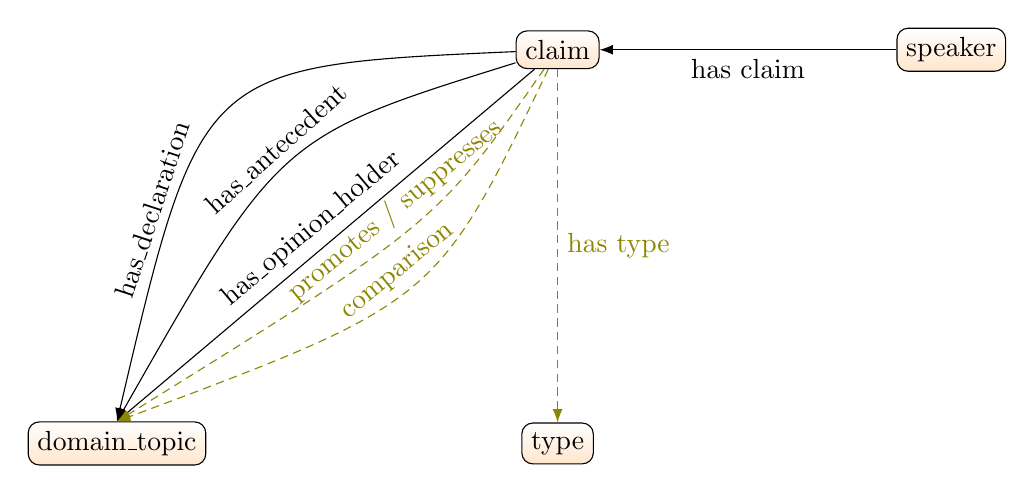
\begin{tikzpicture}[
concept/.style={shape=rectangle, rounded corners,
draw, align=center,
top color=white, bottom color=orange!20},
node distance=5cm,
]
\node[concept] (claim) {claim};
\node[concept, below of=claim] (type) {type};
\node[concept, right of=claim] (speaker) {speaker};
\node[concept, left=4cm  of type] (domain) {domain\_topic};

\draw[-Latex] (speaker) -- (claim) 
	node [midway, below] {has claim}; 

\draw[-Latex, densely dashed, color=olive] (claim) -- (type)
	node [midway, right] {has type}; 

\draw [-Latex] (claim) .. controls ($(claim.west) + (-4cm,
-0.2cm)$) ..  ($(domain.north)$) node [sloped, above, near end] {has\_declaration}; 

\draw [-Latex] (claim) .. controls ($(claim.west) + (-3cm,
-1.1cm)$) ..  ($(domain.north)$) node [sloped, above, midway] {has\_antecedent}; 

\draw [-Latex] (claim) --  ($(domain.north)$) node [above, sloped, midway] {has\_opinion\_holder}; 

\draw [-Latex, densely dashed, color=olive] (claim) .. controls ($(claim.west) + (-1cm,
-2.2cm)$) ..  ($(domain.north)$) node [sloped, above, midway] {promotes / suppresses}; 

\draw [-Latex, densely dashed, color=olive] (claim) .. controls ($(claim.west) + (-1cm,
-3.2cm)$) ..  ($(domain.north)$) node [sloped, above, midway] {comparison}; 

\end{tikzpicture}

\end{document}
